\begin{chapabstract}
\small{
This chapter presents the proposed method to address the real-time source detection problem introduced in \autoref{s:sag}. This chapter is organized as follows. \autoref{s:contribution} will describe the proposed anomaly detection technique. It presents the data pipeline that has been developed to generate input data, the deep learning architectures that have been investigated, and the training process. The evaluation of the models will be addressed in \autoref{s:Experiment-Setup}. \autoref{ss:p-values} will describe the p-value analysis to associate each positive classification with a gaussian statistical significance. \autoref{s:non-stationary-settings} will investigate several problems that can arise during the telescope observations and how those problems can affect the proposed system. 
}\\
\begin{center}
\noindent\makebox[0.8\linewidth]{\rule{0.66\paperwidth}{0.4pt}}
\end{center}
\vspace{1cm}
\end{chapabstract}
\section{The proposed anomaly detection method}
\label{s:contribution}
This section will describe the proposed anomaly detection technique. As explained in \autoref{s:anomaly-detection}, the goal of anomaly detection is the identification of rare items, events, or observations which deviate significantly from the majority of the data and do not conform to a well-defined notion of normal behavior.
This work applies anomaly detection analysis to light curves in the gamma-ray energy spectrum. The y-axis represents the \textit{flux} quantity,  describing how much light a source emits per unit of time and surface. The goal is to identify high-energy phenomena called \textit{Gamma-Ray Bursts} (GRBs), described in \autoref{s:Gamma-Ray-Bursts}. This problem is called \textit{source detection}, and it will be framed into the two  use cases of \textit{serendipitous discoveries} (\autoref{s:serendipitous-discoveries}) and \textit{follow-up observations} (\autoref{s:follow-up-observation}) that require real-time analysis of the data. The problem can be addressed by using an anomaly detection approach considering the \textit{normal data} as the signal coming from a sky region where no sources are present except the background. In contrast, \textit{anomalous data} is defined as the signal coming from a sky region where an astrophysical source is present (along with background).
The proposed method belongs to the model-based family of techniques to detect multivariate sub-sequence anomalies described in \autoref{ss:ad-subsequence-multivariate}. It is based on an autoencoder that learns the time series behavior of normal samples. It thereafter uses reconstruction error as anomaly criteria (\autoref{ss:anomaly-criteria}) to detect anomalies. 
Consider a time series $\bm{X} = \{\bm{x_1}, \bm{x_2}, ..., \bm{x_L}\}$ of length $L$, where each point $\bm{x_i} \in \mathbb{R}^3$ is a 3-dimensional vector of flux values. As we will see in \autoref{ss:data-pipeline}, 
the vector of flux values is composed of logarithmically spaced energy bins between 0.04 and 1 TeV. We consider the scenario where multiple  time series are obtained by taking a window of length $L$ over a larger time series. The autoencoder will be trained on normal samples to minimize the reconstruction error of the decoding step. During the training, the network will learn the model of the background. After training, the autoencoder encodes and decodes data samples and outputs an \textit{anomaly score}. GRBs are then detected as noteworthy deviations from this indicator with respect to the anomaly score of the normal samples. The anomaly score is computed with a weighted mean-squared error to give more importance to prediction errors in the lower energy ranges that contain most of the signal. This is intrinsically due to the source's spectrum, which emits more in the low range of energies. Finally, a sample is classified as an anomaly if the anomaly score is greater than a certain threshold $\tau$. To determine the significance of a GRB detection, the anomaly score is mapped to a p-value through a statistical analysis described in \autoref{ss:p-values}. 

\subsection{The data pipeline}
\label{ss:data-pipeline}
This section will describe the input data and the data pipeline that produces it. As described in \autoref{ss:aperture-photometry} the flux of the electromagnetic radiation emitted by a gamma-ray source can be computed starting from the counts in the on and off regions and the excess counts. The flux measurements can derive a source's spectrum and light curve. The spectrum of a gamma-ray source is a plot of the flux as a function of energy. By measuring the spectrum, astronomers can determine the distribution of energies of the photons emitted by the source and learn about the physical processes responsible for their production. On the other hand, a light curve is a plot of the flux as a function of time. It provides information about how the intensity of the radiation changes over time. The data pipeline developed in this work generates multivariate time series representing light curves for three different energy ranges. The final step of the data pipeline extracts multiple sub-sequences by sliding a window over the light curves. 
A semi-supervised data set of background-only samples is generated at the end of the data pipeline. In particular, for each photon list, several multivariate sub-sequences over three channels are computed. Each sub-sequence point is a flux measurement aggregating one or more seconds of the original photon list. Figure [ref] shows some generated samples. The following sections will explain in detail the components of the data pipeline.

\subsubsection{The photons list simulator module}
\label{ss:dl3-simulator}
The data that is needed for the photometry analysis is produced with simulations. This module aims to simulate the data acquisition of a particular sub-array configuration of CTA, considering its instrument response function (IRF), as described in \autoref{ss:caldb}. The output of the simulation is a photon list. A photon list represents the high-energy photons detected by the telescope sub-array. It is a list that records the detection timestamp for each detected photon, their reconstructed energy, and the direction of arrival with their corresponding errors. Monte Carlo simulation techniques are commonly used to generate these photon lists, as they allow for incorporating various physical processes. The simulator described in \cite{dipiano2022ctasagsci} has been adopted. This is a python package that wraps \textit{ctools}, an open-source community-developed software for the scientific analysis of data from imaging atmospheric Cherenkov telescopes (IACTs), developed in the framework of CTA \cite{Knodlseder_2016}. It has been validated on simulated and real data from H.E.S.S., and Fermi \cite{Knodlseder_2019}. 
Simulations performed with \cite{dipiano2022ctasagsci} can be configured using the following parameters: 
\begin{itemize}
    \item number of simulations (trials): this parameter determines the number of statistically independent realizations under the same conditions. The only difference between the trials is the seed, making the trials statistically independent.
    \item simulation duration (tobs): this parameter determines the duration of the observation in seconds.
    \item minimum energy, maximum energy, and region-of-interest's size (emin, emax, roi): these parameters constrain the output of the simulation. The gamma-ray photon will have energy in the range $[EMIN, EMAX]$ (expressed in TeV), and their direction of arrival will be inside the region of interest (ROI), a circular region inside the field-of-view, whose radius is expressed in degrees.
    \item simulation type (simtype): this parameter is used to decide which models the simulation will consider: in a background-only simulation, only the background model is used. In a GRB simulation, only the GRB models are considered (check the next bullet point). In addition, the results of background and GRB simulations can be merged together to generate a photon list containing both.  
    \item GRB template (runid): this parameter is needed to simulate a GRB event. As outlined in \autoref{s:Gamma-Ray-Bursts}, the GRBs events are different in terms of duration and luminosity, and the template is a model of the evolutionary process of the event. It is a 3-dimensional grid of fluxes, 70 temporal bins, and 40 energy bins. Hence, the template defines 70 light curves for each energy bin, and for each light curve, it defines 40 spectra. The simulation will integrate the light curve and the spectra within a time-energy interval in the 2D space of a sky map considering the XML spatial model (RA, DEC) of the point-like source. The templates used in this work are taken from the POSyTIVE catalog. The mock GRB population used by POSyTIVE is calibrated using a 40-year data set of multi-wavelength GRB observations \cite{Bernardini_2019}.
    \item GRB start (onset): the delay in seconds between the start of the observation and the start of the GRB event.
    \item GRB displacement from on-axis (offset): this parameter is the offset (in degrees) added to the on-axis pointing that represents the position of the simulated source. The value of this parameter is considered fixed and equal to $0.5\degree$ for all simulations. 
    \item instrument response function (irf): different types of telescopes and array configurations have different IRFs. Only one IRF has been used to run all simulations, i.e., $North\_z40\_5h\_LST$ which models the response of a sub-array composed of 4 LST-1 telescopes located in the northern hemisphere site, observing for 5 hours at $40^{\circ}$ zenith angle. This IRF has been chosen to model extra-galactic observations. Simulated galactic plane observations would require both the diffuse emission and known source models that are not available at the time of writing. Only one IRF has been considered because the GRBs catalog doesn't contain the \textit{trigger times}, i.e., the timestamp associated with the start of the GRB events. Without this temporal reference is not possible to infer the position of the GRBs. Hence, they are all simulated in the same sky region. A single IRF is sufficient because only one background level is considered, observing at $40\degree$  zenith angle, an intermediate case between the zenith and the horizon.
    \item Calibration database (caldb): this database contains CTA's instrument response functions (IRFs), described in \autoref{ss:caldb}. The calibration database used in this work is tagged by version \textit{prod5 v0.1} \cite{zenodo_2021}.
\end{itemize}
In order to simulate GRB events, the extra-galactic background light (EBL) must be considered. This is the integrated intensity of all the light emitted throughout the universe's history across the entire electromagnetic spectrum \cite{Cooray_2016}. 
If the involved photon energies are above the threshold for electron-positron pair creation, very high energy gamma-rays ($E >100 GeV$) are absorbed from the EBL through interaction with low-energy photons \cite{Mazin_2013}. The simulator \cite{dipiano2022ctasagsci} accounts for the EBL absorption, extracting the power law spectral models from the templates and modifying them by applying an exponential cutoff with a predefined absorption level \cite{Gilmore_2012}. Finally, it generates new light curves considering the new absorbed spectral models. 
To speed up the simulation process, the python code of the simulation script has been rewritten to support batch parallelization with SLURM. The output of the simulations is a set of photon lists in Flexible Image Transport System (FITS) format, the standard data format used in astronomy. It is used for transporting, analyzing, and archival storing scientific data sets, supporting multi-dimensional arrays. A FITS file contains one or more tables with rows and columns of information and a header containing metadata \cite{fitswebsite}. A photon list contains all the detected photons, described by the detection timestamp, their reconstructed energy, and the direction of arrival.
It is important to highlight that although the photon list generation is the most resources intensive process in this work, it can be executed only once for each IRF. Several photometry analyses with different integration times can be performed from this data set.

\subsubsection{Photometry module}
\label{ss:photometry-module}
This software module takes as input the photon lists generated by the simulator, along with several other parameters. It integrates the gamma-ray photons along three dimensions: space, time, and energy. For each photon list as input, it generates a multivariate time series of flux values. This software module has been built on the work of \cite{tampieri2020real}, wrapping the region counting routine and the effective area computation. The rest of this software module has been developed to optimize the computations' speed as much as possible. 
The public API is represented by the \textit{OnlinePhotometry} class, which accepts the parameters used in the simulation process and the following configuration parameters. The \textit{integration time} (itime) defines the size of the temporal bins used for the time integration of the photon list. For example, with 500 seconds of observation and an integration time of 5 seconds, we obtain $500/5=100$ points representing a time series of photon counts. The \textit{number of energy bins} that is used to compute the energy bins, logarithmically spaced between $tmin=0.04 TeV$ and $tmax=1 TeV$. Considering more than one energy bin, the integration process will output a multivariate time series of photon counts, dividing the photons in each energy bin. In the latter example, the output data shape would equal $(100,3)$. Finally, the \textit{sub-window size} (sws) parameter truncates the time series to have \textit{sws} points. In the latter example, the output shape would be $(0:sws, 3)$. After defining the temporal end energy integration parameters, the spatial dimension must also be defined. As outlined in \autoref{ss:aperture-photometry}, the spatial region is a circular sky region defined by a center in sky coordinates and a radius expressed in degrees. Only the photons whose arrival direction falls into the circular region are counted. The circle's center is defined by adding an offset in degrees from the pointing. The pointing is read from the header of the FITS file. At the same time, the center of the region is computed automatically with a predefined offset added to the on-axis pointing direction. This is accomplished by providing the parameters \textit{regions\_radius} and \textit{max\_offset} to the \textit{integrate} method. To avoid underestimating or overestimating the photon counts, the value of the \textit{regions\_radius} should be equal to the instrument's point spread function (PSF). Still, since the PSF size depends on the energy range, three different region sizes would have been considered. To avoid this complexity, we assumed a fixed value of $0.2\degree$, also because the core of the photometry tool \cite{tampieri2020real} corrects the photon count by a scaling factor proportional to the PSF size. The last step is to transform the time series of photon counts into flux values. The flux ($\Phi$) in $ph\,cm^{-2}\,s^{-1}$ is defined by
$$
\Phi(E)=\frac{dF}{dE}(E)=\frac{dN_\gamma}{dE\,\,dA_{eff}\,\,dt_{eff}}
$$
where $dN_\gamma$ is the number of excess events in $dE$ energy, $A_{eff}$ is the \textit{effective area} in the chosen source region and $t_{eff}$ is the effective observation time. The effective area $A_{eff}(\theta,E_\gamma)$ is the geometric area where photons are collected, multiplied by an efficiency term that depends on the energy of the incoming photons and its angular distance $\theta$ from the optimal on-axis pointing direction. The CTA observatory has a higher effective area in the high-energy range, but it degrades slowly with respect to the pointing-source angle \cite{tampieri2020real}. Since the $\Phi(E)$ formula normalizes the photon counts for the effective area, taking into account the degradation of the IRF, which increases while moving away from the telescope's pointing, it's possible to extract the photon counts from multiple regions with different offsets from the optimal on-axis pointing direction. Extracting flux measurements from multiple regions in the sky simultaneously significantly boosts the data generation rate and the field-of-view coverage.
The \textit{OnlinePhotometry} class uses the \textit{RegionsConfig} class, which responsibilities are the computation of the regions' position and their effective area. As stated at the beginning of this section, this software module has been developed to optimize the computations' speed as much as possible. The effective area must be computed for each region and each energy bin. However, if multiple photon lists have been simulated using the same IRF, the effective area can be computed only once for the first photon list and then reused. \textit{OnlinePhotometry} has a \textit{preconfigure\_regions} method that performs this computation. If this method is not called, the \textit{integrate} method will compute the effective area for each photon list.

Another optimization trick is to consider a ring of regions, i.e., all regions that share the same distance from the on-axis pointing. The effective area computation for this group of regions can be done only once since the $\theta$ angle does not change. \autoref{fig:rings} shows an example of multiple ring regions produced by the \textit{RegionsConfig} class. The white region is centered on the source.
\begin{figure}[t]
\centering
\includesvg[width=0.9\linewidth]{figures/method/rings.svg}
\caption{An example of the rings regions produced by the \textit{RegionsConfig} class. The white region is centered on the source.}
\label{fig:rings}
\end{figure}


\subsubsection{Time series extractor module}
\label{ss:extractor}
The last step of the data generation pipeline is to apply a time series extractor module to extract sub-sequences from the time series generated by the previous step. A sub-window of length \textit{sws} slides over the original time series with a specific \textit{stride}, i.e., the distance the sub-window moves at each step. The number of sub-sequences the method will extract is dependent on the chosen length (i.e., the shorter the length, the higher the number of sub-sequences) and the chosen \textit{stride} (i.e., the shorter the \textit{stride}, the higher the number of sub-sequences). To generate the train set the value of the stride can be arbitrary since the training is performed offline. In \autoref{ss:p-values} we will require our samples to be statistically independent, meaning no overlapping among the sub-sequences. This can be accomplished by setting the value of the \textit{stride} equal to the \textit{sws}. In contrast, during inference, we will need to increase the sample rate generation to increase the inference rate, so a \textit{stride} equal to one is preferred. 

As stated before, a semi-supervised data set of background-only samples is generated at the end of the data pipeline. In particular, for each photon list, several multivariate sub-sequences of length \textit{sws}, over three channels, are computed. Each sub-sequence point is a flux measurement aggregating $itime$ seconds of the original photon list.  


\subsection{Autoencoder architectures}
\label{ss:architectures}
As outlined in \autoref{s:contribution}, the proposed method belongs to the model-based family of techniques to detect multivariate sub-sequence anomalies. It is based on an autoencoder that learns the time series behavior of normal samples. It thereafter uses reconstruction error as anomaly criteria to detect anomalies. 
The architecture of an autoencoder can exploit different types of layers. A convolutional autoencoder typically consists of multiple layers of convolutional and pooling operations. It allows the network to learn spatial hierarchies of features. On the other hand, an autoencoder implemented with recurrent layers is designed to process data sequences, such as text or time series. The autoencoder can learn temporal dependencies and patterns in sequential data with recurrent layers. As mentioned in \autoref{s:ad-with-dl}, more complex and hybrid architectures have been developed such as Temporal Convolutional Networks to  make a CNN layer to understand patterns that occur over a prolonged period \cite{Lea_2016}, ConvLSTM to address the spatio-temporal sequence-forecasting problem \cite{Shi_2015} and transformer (BERT), that implements the current state-of-the-art architectures \cite{Devlin_2018}. In this work, two types of autoencoder architectures have been investigated, based on CNN, and RNN layers, resulting in different performance outcomes, both in terms of false positive minimization and training requirements. The architecture has been kept small, with no more than four layers and a few thousand learnable parameters. Since the input data has a low dimensionality, too much complex architecture will be able to memorize and overfit the training data. For the same reason, dropout layers are applied in each model architecture. The dropout layer randomly sets input units to 0 with a certain frequency (20\% in this case) at each step during training time, which helps prevent overfitting. More complex architectures have not been considered because of the low dimensionality of the input. In particular, LSTM layers have not been considered because they're not long-term temporal dependencies in the input data. 

\subsection{Autoencoder training}
\label{ss:training}
As stated in \autoref{s:anomaly-detection}, the autoencoder is trained in a semi-supervised setting to learn the time series behavior of normal samples. A semi-supervised data set of background-only time series has been generated using the data processing pipeline described in \autoref{ss:data-pipeline}. According to the Science Alert Generation (SAG) design requirements (\autoref{ss:sag-requirements}), the real-time search for transient events should be performed on multiple time scales. The \textit{integration time} setting is used to vary the time scale, integrating the photon counts in tighter or wider time bins. In \cite{tampieri2020real}, and \cite{di2021detection}, the authors explore the capabilities of the Li\&Ma and Full-FoV Maximum Likelihood in the short exposure scenario, using very short integration times. The proposed technique is tested under the same extreme setting. In particular, two training data sets have been used, with integration times equal to 5 seconds and 1 second. I will refer to the first data set as \textit{short-exposure analysis} and to the second data set as \textit{very short-exposure analysis}. As mentioned in \autoref{ss:photometry-module}, the photon lists can be generated and written to the file system as FITS file only once (unless we want to change the simulation parameters, such as the IRF). Then, using the \textit{OnlinePhotometry} class introduced in \autoref{ss:photometry-module}, several data sets of multivariate time series can be generated. A \textit{DataManager} class has been developed to manage the data used for the autoencoder training and testing. It wraps the \textit{OnlinePhotometry} class to generate the multivariate time series of flux values, extracting the photon counts from multiple regions and applying normalization. This class implements a caching feature to avoid repeating the previous computation multiple times. Finally, it exposes a \textit{get\_train\_set} method to apply all the required data pre-processing to generate training data. In particular, the first step is to extract sub-sequences from the time series. The stride value is equal to 5 to obtain sub-sequences that do not overlap, but shorter strides could be used. The sub-sequences samples are then split into train and validation sets. A MinMax scaler is fitted on the train set and applied to it, scaling the samples to the $[0, 1]$ interval with the formula $ \frac{x-min(x)}{max(x)-min(x)}$. \autoref{tab:training-set-fits} summarizes the simulation parameters to generate the FITS data set, and \autoref{tab:training-set-ts} summarizes the parameters to generate the train set. The resulting samples in the short-exposure and very short-exposure settings are, respectively, 48960 for training, 12240 for validation, and 68000 for training, 17000 for validation. 
\begin{table}[]
\centering
\begin{tabular}{|l|l|}
\hline
\multicolumn{2}{|c|}{\textbf{Simulation parameters}} \\
\hline
trials          & 10                  \\ 
simtype         & bkg                 \\ 
runid           & run0406\_ID000126   \\ 
scalefluxfactor & 1.0                 \\ 
caldb           & prod5-v0.1          \\ 
emin            & 0.04                \\ 
emax            & 1                   \\ 
irf             & North\_z40\_5h\_LST \\ 
offset          & $0.5\degree$                \\ 
roi             & $2.5\degree$                 \\ 
tobs            & 18000               \\ \hline
\end{tabular}
\caption{The parameters used to customize the photon lists simulation for the train set generation.}
\label{tab:training-set-fits}
\end{table}
\begin{table}[]
\centering
\begin{tabular}{|l|l|}
\hline
\multicolumn{2}{|c|}{\textbf{Train test (short-exposure)}} \\
\hline
integration\_time  & 5 \\ 
number\_of\_energy\_bins & 3 \\ 
normalize & True \\ 
sub\_window\_size & 5 \\ 
stride & 5 \\ 
validation\_split & 80\% \\ 
Train samples & 48960 \\ 
Validation samples & 12240 \\ \hline
\end{tabular}
\quad
\begin{tabular}{|l|l|}
\hline
\multicolumn{2}{|c|}{\textbf{Train test (very short-exposure)}} \\
\hline
integration\_time  & 1 \\ 
number\_of\_energy\_bins & 3 \\ 
normalize & True \\ 
sub\_window\_size & 5 \\ 
stride & 5 \\ 
validation\_split & 80\% \\
Train samples & 68000 \\ 
Validation samples & 17000 \\ \hline
\end{tabular}
\caption{The parameters used to configure the \textit{DataManager} class to extract sub-sequences with photometry and to generate the training set. The left panel shows the parameters of the short-exposure scenario, while the right panel shows the parameters of the very short-exposure scenario.}
\label{tab:training-set-ts}
\end{table}

The autoencoders have been trained with the \textit{Adam} optimization \cite{Kingma_2014} and a \textit{learning rate} of 0.0001. A 20\% dropout is applied after each layer. As shown by \autoref{tab:training-set-ts}, 80\% of the samples are used for training, while the remaining 20\% is set aside for validation. As already mentioned, the inputs are scaled to the $[0, 1]$ interval. The \textit{batch size} has been set to 32 samples. The autoencoder \textit{loss} (or \textit{anomaly score}) is a \textit{weighted mean squared error} (MSE), defined as the following:
\begin{definition} \label{def:wmse}
[Weighted MSE] $\textbf{WMSE}=\frac{1}{2D}\sum_{i=1}^{D}\bm{w}(\bm{x_i}-\bm{y_i})^2$ where $\bm{w}=[\frac{1}{2}, \frac{1}{3}, \frac{1}{6}]$ and D is equal to the number of points. 
\end{definition}
The reason behind this choice is to give more importance to prediction errors in the lower energy ranges that contain most of the signal. An \textit{early stopping} strategy was considered during training, but the \textit{validation loss} was already flat after five epochs for all models. Hence, the models' weights have been written on disk after five epochs of training. \autoref{fig:train-val-loss-itime-5} shows the training and validation losses for the autoencoder with recurrent layers trained in the short-exposure scenario. More results can be found in \autoref{s:appendix-b}.
\begin{figure}[t]
    \centering
    \begin{minipage}{1\textwidth}
       \centering
        \includesvg[width=\linewidth]{figures/method/training/AnomalyDetector_rnn_l2_u32_train_val_loss_itime_5}
    \end{minipage}
    \caption{An example of train loss and validation loss for the autoencoder with recurrent layers in the short-exposure scenario (integration time = 5 seconds).}
    \label{fig:train-val-loss-itime-5}
\end{figure}
 


\section{P-value analysis}
\label{ss:p-values}
As outlined in \autoref{ss:sag-requirements}, the Science Alert Generation (SAG) system must be able to generate candidate science alerts, meaning that the positive classification produced by the proposed system must be associated with a gaussian $\sigma$ level of statistical significance. A statistical pipeline based on hypothesis testing has been developed to achieve that. This analysis is used to obtain the threshold $\tau$ to classify the samples as anomalies with a certain $\sigma$ level (\cite{Parmiggiani_2021}) or, on the contrary, to associate with each anomaly score a statistical confidence level (of a positive classification). 
\begin{figure}[t]
\centering
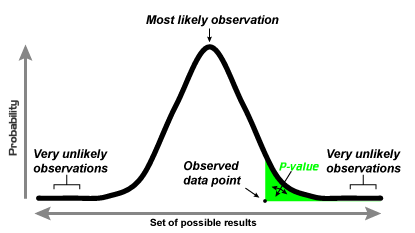
\includegraphics[width=0.6\linewidth]{figures/method/pvalue.png}
\caption{A one-tailed test, showing the p-value as the size of one tail. Credits to \url{https://en.wikipedia.org/wiki/One-_and_two-tailed_tests}}
\label{fig:p-val-one-tailed}
\end{figure}
In hypothesis testing, the initial assumption is that there is no correlation between the predictor and outcome variables in the population. Through statistical tests utilizing collected data, a determination is made as to whether there is enough evidence to reject the null hypothesis in favor of the alternative hypothesis. A two-tailed hypothesis test is designed to show whether the measure is significantly greater than and significantly less than the mean of a population. The two-tailed test gets its name from testing the area under both tails (sides) of a normal distribution. On the other hand, a one-tailed hypothesis test is set up to show that the measure would be higher or lower than the population mean. \autoref{fig:p-val-one-tailed} illustrates a one-tailed test, showing the p-value as the size of one tail. The level of statistical significance, represented by p-values, serves as the benchmark for these tests. The p-value is the likelihood of obtaining the study results by chance if the null hypothesis is true.
\begin{definition}
\label{def:pvalues} 
The p-value is the inverse of the cumulative distribution function of the test statistic. it defines the probability of accepting the alternate hypothesis with a given level of statistical confidence where in fact the null hypothesis is true:
$$ p(ts \geq h) = \int_{h}^{\infty} \phi(x) \,dx $$
where $ts$ is the test statistic of the experiment, $\phi$ is the distribution of the test statistic of the observed experiments, and $h$ is a threshold.
\end{definition}
In other words, the p-value is the likelihood of committing a type I error (false-positive) if one rejects a null hypothesis that is actually true. On the contrary, a type II error (false-negative) occurs if one fails to reject a null hypothesis that is actually false.
The null hypothesis is rejected in favor of the alternative hypothesis if the p-value is less than the established level of statistical significance. 
For example, we can reject the null hypothesis if the p-value is less than $3x10^{-7}$ meaning $> 5\sigma$ confidence in the alternative hypothesis. 
Results with p-values lower than $3x10^{-7}$ can still be false positives every once in $3x10^7$ measures ($\pm$ statistical fluctuations). A metric that considers the number of false positives (or false alarms) per the total number of times the event didn't happen is called \textit{false alarm rate} (FAR). A false alarm rate is also known as the probability of false detection. To not be confused with the false alarm ratio (also abbreviated as FAR), which is the number of false alarms per the total number of warnings or alarms. Regarding hypothesis testing, if P is the probability of committing a type I error (rejecting the null hypothesis when it is actually true) and Q is the probability of making a type II error (failing to reject the null hypothesis when it is actually false), in this study, we prioritize minimizing Q over P to minimize the false positive rate and prevent the system from issuing false science alerts to the scientific community. 

The null hypothesis in this context is represented by the absence of the GRB event in the data. The anomaly score is the test statistic considered in the p-value analysis. To evaluate the p-values, a data set composed of background-only data samples is fed to the autoencoder, and the distribution $\phi$ of the corresponding anomaly scores is computed. Then, the inverse of the cumulative distribution function is evaluated, obtaining a mapping between the test statistics and the p-values. As stated before, a p-value defines the probability of obtaining statistical confidence greater or equal to a threshold $h$ when the null hypothesis is true. 

To reach the desired $5\sigma$ level, about $1e^8$ trials need to be simulated and transformed into sub-sequences fed to the autoencoder to obtain the anomaly scores. The same simulation settings are used to generate the training test for the autoencoder models. Hence, more details about the data set generation for the p-value analysis will be provided in \autoref{ss:training}. There're only two differences concerning the simulation parameters used to generate the training set: the observation time is limited to 100 seconds, and the number of simulated trials is $1e^8$. This process is very computing intensive and has to be repeated several times each time a new model is deployed in production. The latter number is why the simulation script provided by \cite{dipiano2022ctasagsci} has been improved and optimized. As outlined in \autoref{ss:dl3-simulator}, starting from this data set, it is possible to perform different photometry analyses and extract sub-sequences with different lengths. For this reason, a script exploiting batch parallelization with Slurm has been developed to load a trained autoencoder, apply the photometry analysis, generate the sub-sequences, and perform inferences. In particular, each Slurm job takes a batch of photon lists, integrates the photon counts, computes the flux, extracts the time series, scales the data, and performs inference, measuring the anomaly score. In order to guarantee the statistical independence of these measures, from each photon list, only one sub-sequence is generated and given to the autoencoder. This is why the observation time was limited to 100 seconds. The time took to process $1e^7$ trials (about $3.5 TB$ of data), using 100 jobs on 60 Intel(R) Xeon(R) Gold 6240 CPU  cores, was about 48 hours. The computational bottleneck was due to the network filesystem that limited the data transfer from a SATA hard drive. 

In order to find the corresponding p-value for a given sigma level, first of all, we defined the two-tailed probability corresponding to the sigma level of choice. For example, if $sigma=3$, the corresponding two-tailed probability is $p=99.73\%$. The p-value is given by the survival function: $(1-p)=0.0027$. This p-value describes the probability of having a measure outside the  $\pm3\sigma$. Since this use case is constructed on half of a symmetrical distribution, the one-tailed p-value of that probability must be computed. Hence, the previous p-value must be halved, obtaining $(1-p)/2=0.00135$. The p-value is then mapped to a threshold value. On the contrary, if we want to know the sigma level of a particular threshold, we take the corresponding p-value and find the inverse cumulative distribution function relative to that p-value. Again, since the normal distribution is symmetrical, the absolute value is the number of standard deviations rather than  $\pm n\sigma$. if the threshold value is not present in the table, it can be interpolated within the closest two values along with the corresponding p-values interpolation.  

%%%%%%%%%%%%%%%%%%%%%%%%%%%%%%%%%
% QUESTA PARTE E' DA FINIRE
%%%%%%%%%%%%%%%%%%%%%%%%%%%%%%%%%

\section{Inference}
\label{ss:inference}

% Plot predictions not anomalous and anomalous
% SI ottiene MSE
% Si calcola sigma
% Si ripete fino alla fine della timeseries
\autoref{fig:cnn-predictions-itime-5}

\begin{figure}[!htb]
\centering
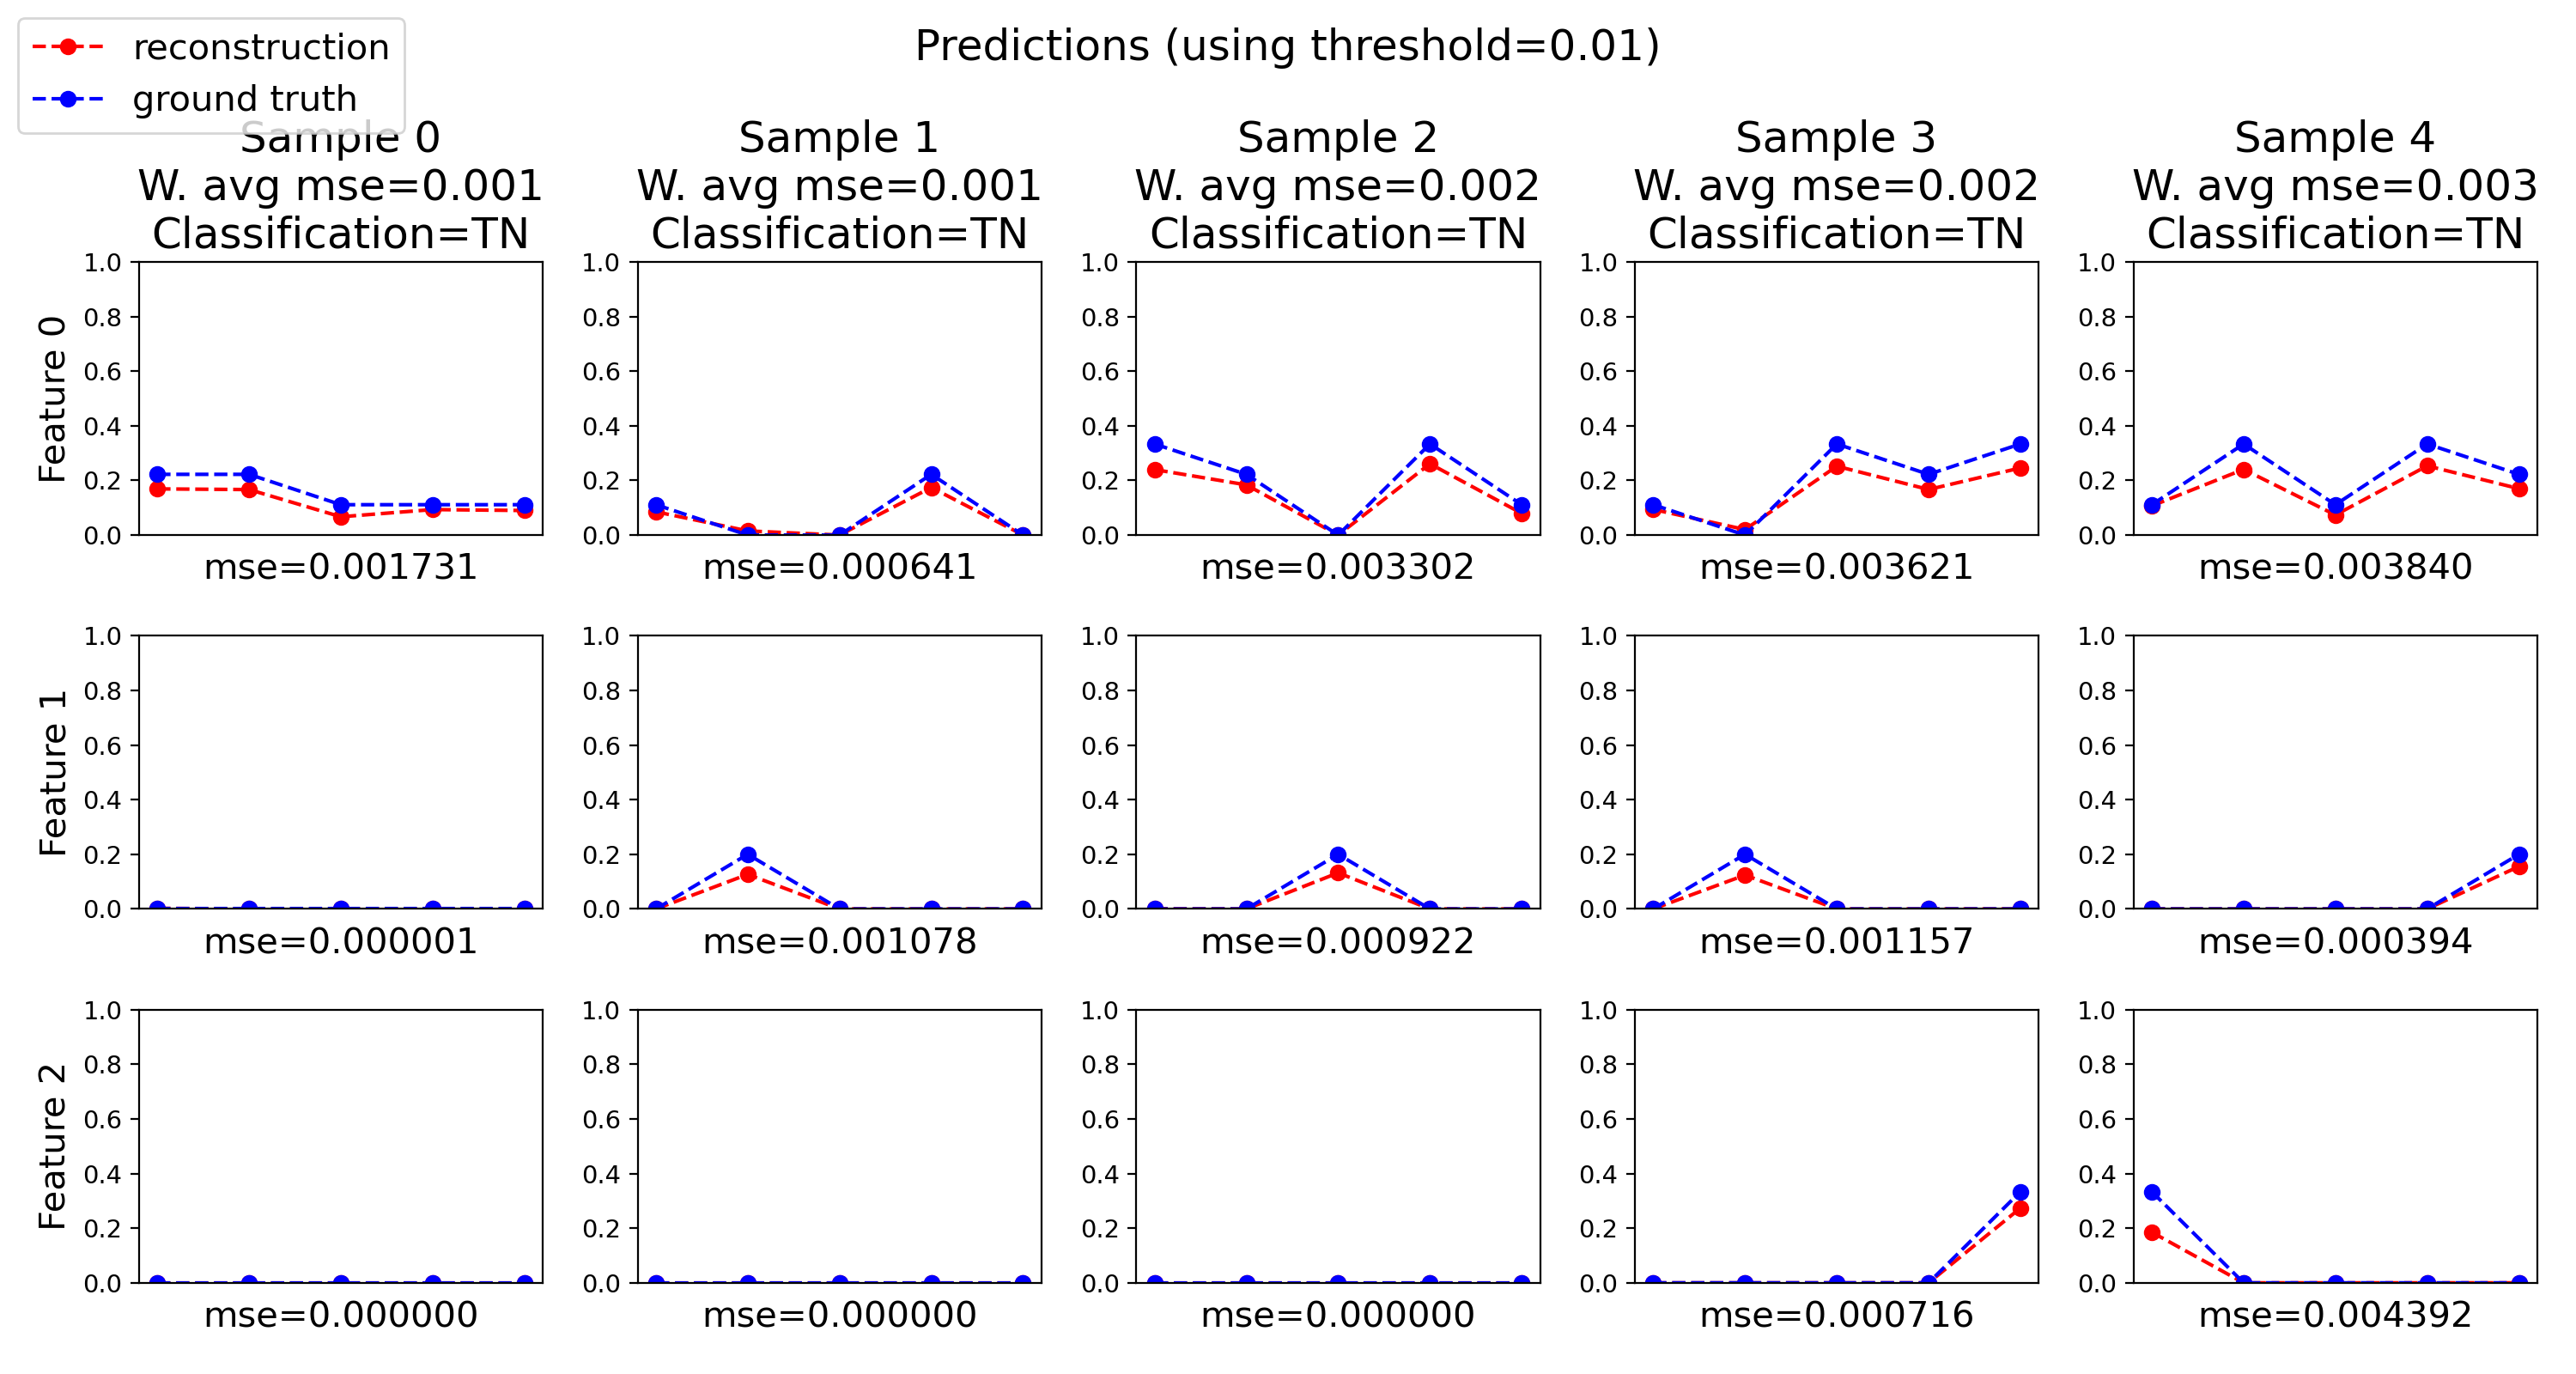
\includegraphics[width=\linewidth]{figures/training/cnn_epoch_5_plot_0_predictions_itime_5.png}
\caption{ }
\label{fig:cnn-predictions-itime-5}
\end{figure}

\begin{figure}[!htb]
\centering
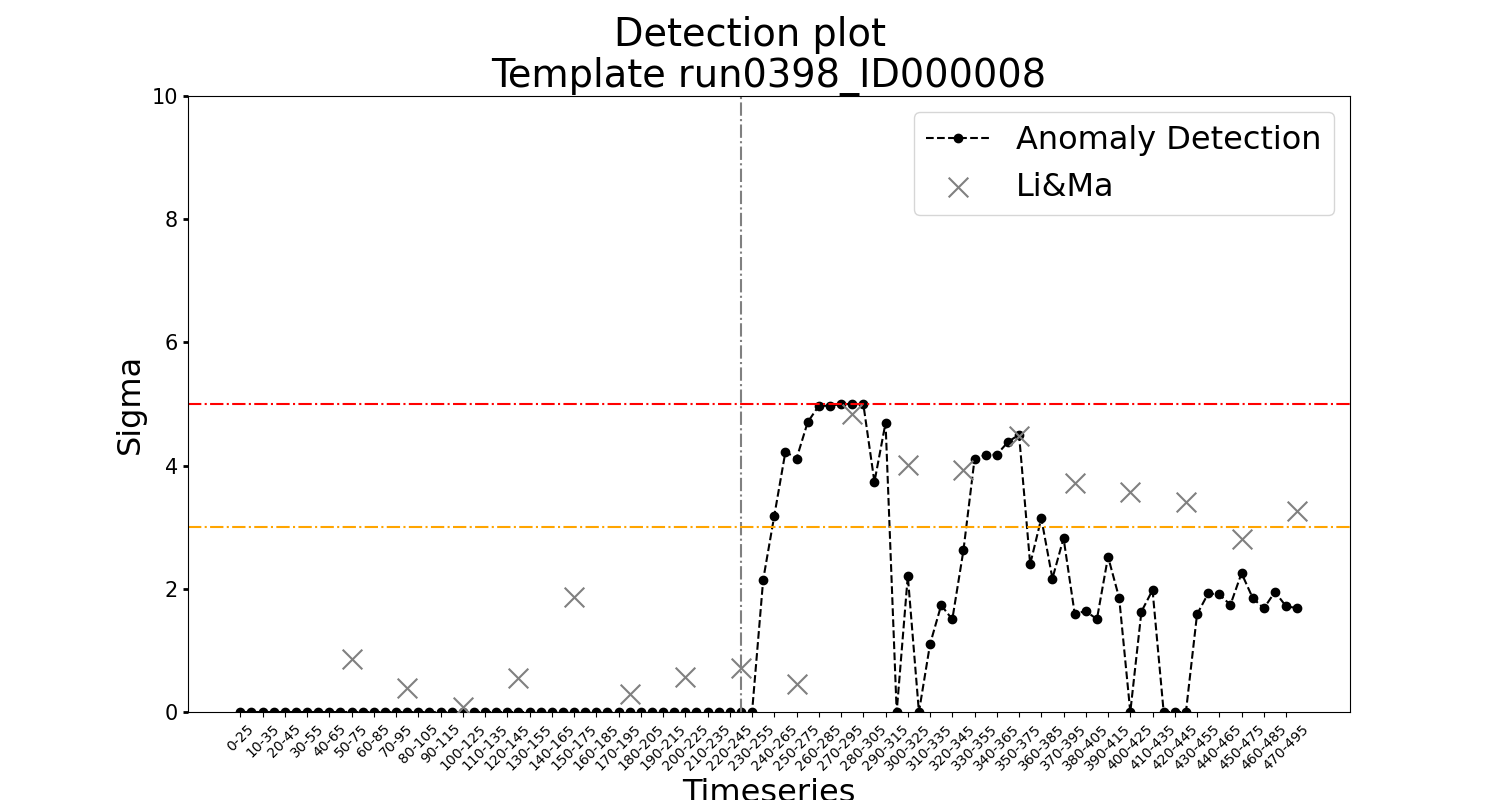
\includegraphics[width=\linewidth]{figures/experiments/detection_plots/detection_plot_run0398_ID000008_testset_e.png}
\caption{ }
\label{fig:detection_plot}
\end{figure}



\section{System design}
\label{s:system-design}

\begin{figure}[!htb]
\centering
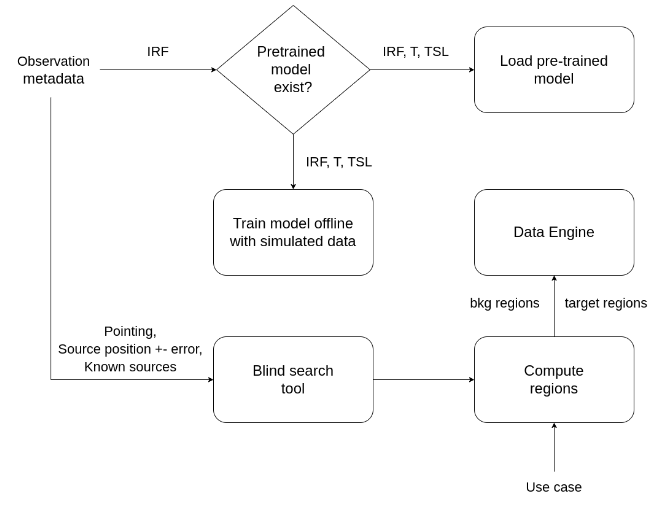
\includegraphics[width=\linewidth]{figures/method/systemdesign1.png}
\caption{ }
\label{fig:system-design-1}
\end{figure}

\section{Non-stationary settings}
\label{s:non-stationary-settings}
During inference, the model will process the real-time data generated by the telescopes during an observation. As explained in \autoref{s:anomaly-detection}, the stationarity property of the stochastic process that generates the data can be invalidated by concept drifts. This can be a significant issue as it can negatively impact the performance of a machine learning model trained under a certain statistical distribution of input data. Neural networks are particularly vulnerable to concept drift, as they rely on the assumption that the data distribution remains constant during training and inference. In the presence of a concept drift, the model makes predictions based on outdated information, leading to decreased accuracy. 





\section{Summary}
The previous chapter proposed a method to address the real-time source detection problem. The contribution described the anomaly detection technique, including the data pipeline for input generation, the investigated deep learning architectures, and the training process. The evaluation of the models was addressed in the experiment setup section. The p-value analysis was described to associate positive classifications with gaussian statistical significance. The potential problems of non-stationary settings during telescope observations and their impact on the proposed system were investigated.